\documentclass{article}
\usepackage[
        a4paper,% other options: a3paper, a5paper, etc
        left=3cm,
        right=3cm,
        top=3cm,
        bottom=4cm,
        % use vmargin=2cm to make vertical margins equal to 2cm.
        % us  hmargin=3cm to make horizontal margins equal to 3cm.
        % use margin=3cm to make all margins  equal to 3cm.
]{geometry}
%\usepackage[utf8x]{inputenc}
\usepackage{graphicx}
\usepackage{caption}
\usepackage{enumerate}
\usepackage{subcaption}
\usepackage[procnames]{listings}
\usepackage{color}
\usepackage{amssymb}
\usepackage{amsmath}
\usepackage{comment}
\usepackage{hyperref}
\usepackage{blindtext}
\usepackage[titletoc,title]{appendix}
\usepackage{float}
\usepackage{fullpage}
\definecolor{codegreen}{rgb}{0,0.6,0}
\definecolor{codegray}{rgb}{0.5,0.5,0.5}
\definecolor{codepurple}{rgb}{0.58,0,0.82}
\definecolor{backcolour}{rgb}{0.95,0.95,0.92}

\lstdefinestyle{mystyle}{
    backgroundcolor=\color{backcolour},
    commentstyle=\color{codegreen},
    keywordstyle=\color{magenta},
    numberstyle=\tiny\color{codegray},
    stringstyle=\color{codepurple},
    basicstyle=\ttfamily,
    breakatwhitespace=false,
    breaklines=true,
    captionpos=t,
    keepspaces=true,
    numbers=left,
    numbersep=5pt,
    showspaces=false,
    showstringspaces=false,
    showtabs=false,
    tabsize=2
}

\lstset{style=mystyle, language=Matlab}
\renewcommand{\thesubsection}{\small(\alph{subsection})}

\title{Signals and Systems Lab 2}
\author{Maikel Withagen (s1867733) \and Steven Bosch (s1861948)}
\date{\today}

\begin{document}
\maketitle

\section{Time delay and correlators}
\subsection{}
See section \ref{code:1a} in the appendix for our implementation of the function $circorr$.

\subsection{}
Figure \ref{fig:1b1} gives the discrete random signal x and figure \ref{fig:1b2} gives the circular correlation between x and itself. Our conclusion is that at a delay of 0 (index of 1) the circular correlation is 1, which is logical because at a delay of 0 the signals are equal. Because the signal $x$ is randomly generated, any other delay will result in a low correlation.
\begin{figure}[H]
	\centering
	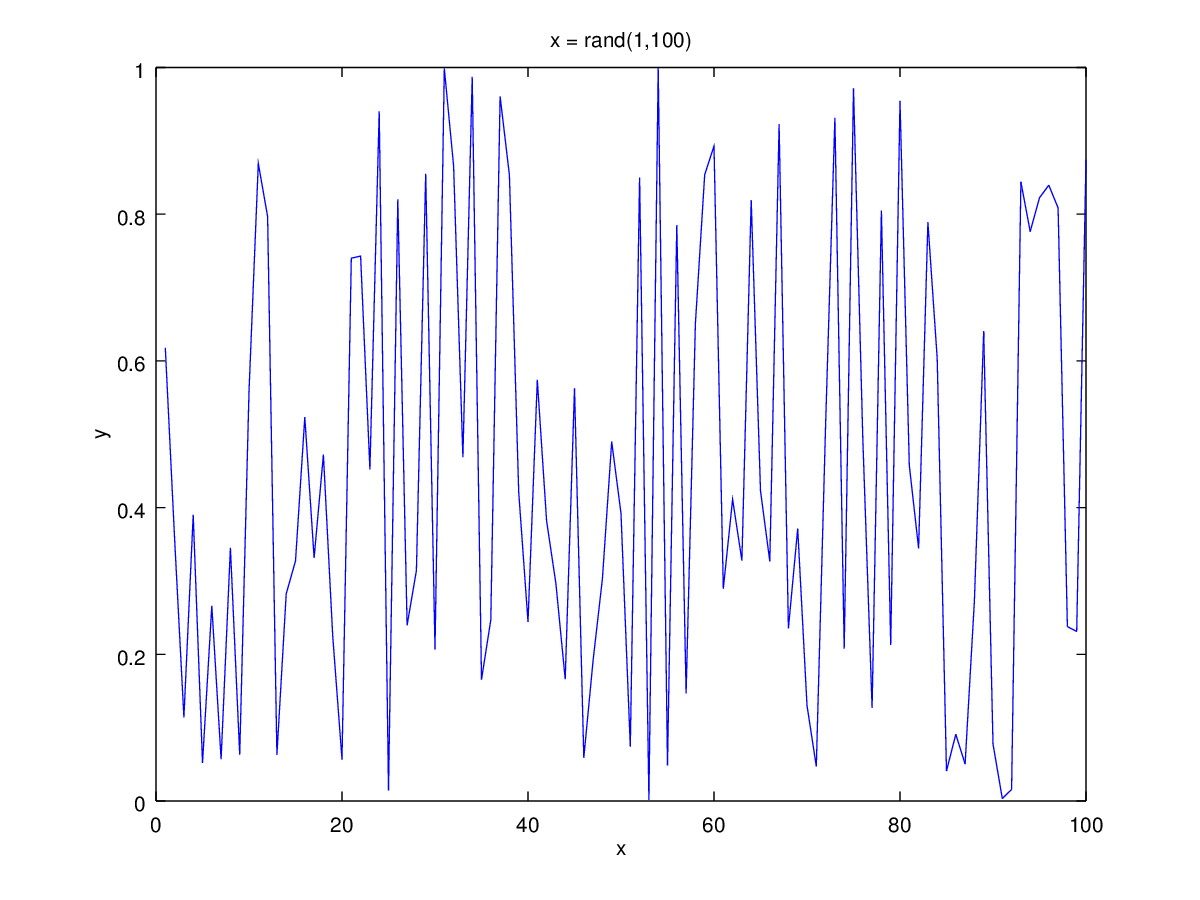
\includegraphics[width=.7\textwidth]{plot1b1.png}
	\caption{The function $x$.}
	\label{fig:1b1}
\end{figure}
\begin{figure}[H]
	\centering
	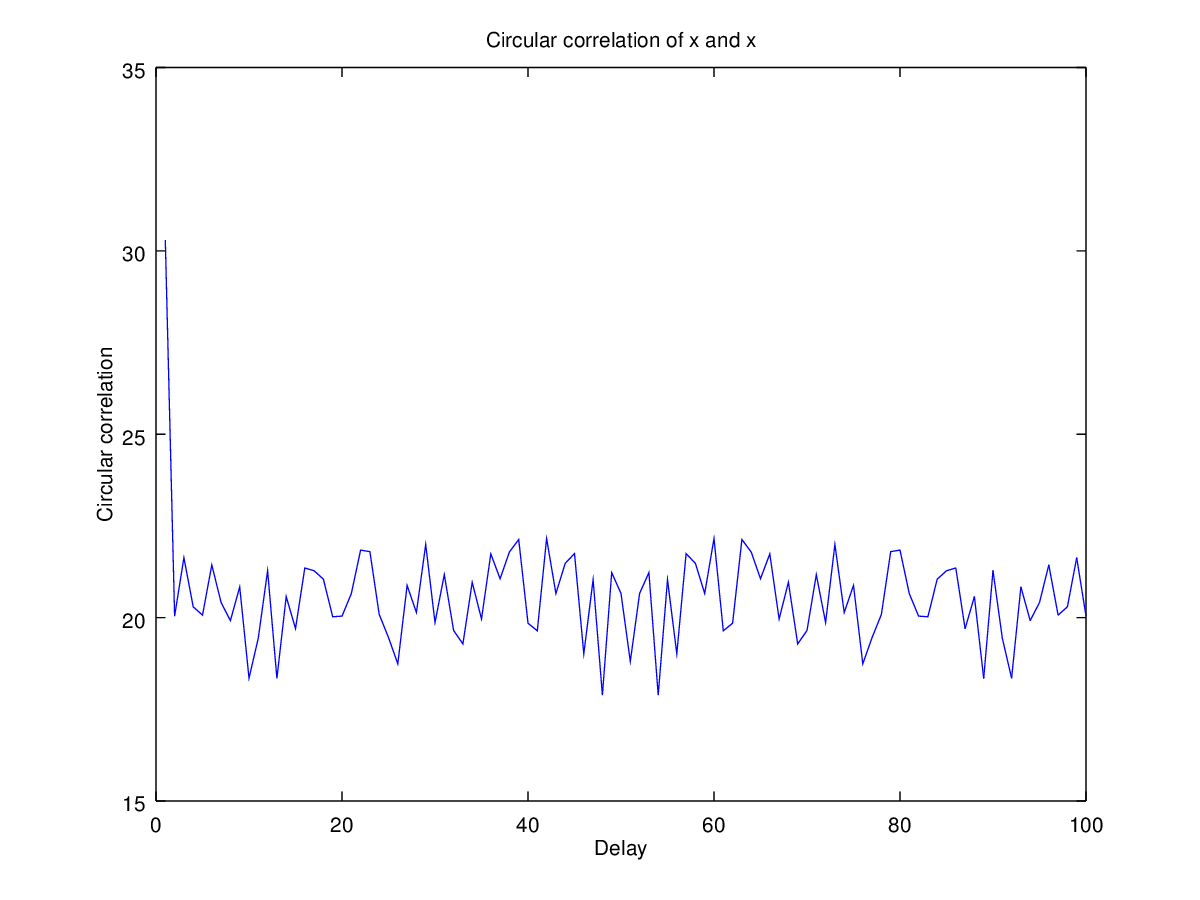
\includegraphics[width=.7\textwidth]{plot1b2.png}
	\caption{The circular correlation between $x$ and itself.}
	\label{fig:1b2}
\end{figure}

\subsection{}
See section \ref{code:1c} in the appendix for our implementation of the function $rotate$. Figure \ref{fig:1c} gives the plot of the circular correlation between $x$ and $y$. As we can see, the peak has shifted to a delay of 50. This was to be expected, since we shifted $x$ 50 places to construct $y$. So effectively, the circular correlation between $x$ and $y-50$ is equal to the correlation between $x$ and itself (which can be observed in the previous section).
\begin{figure}[H]
	\centering
	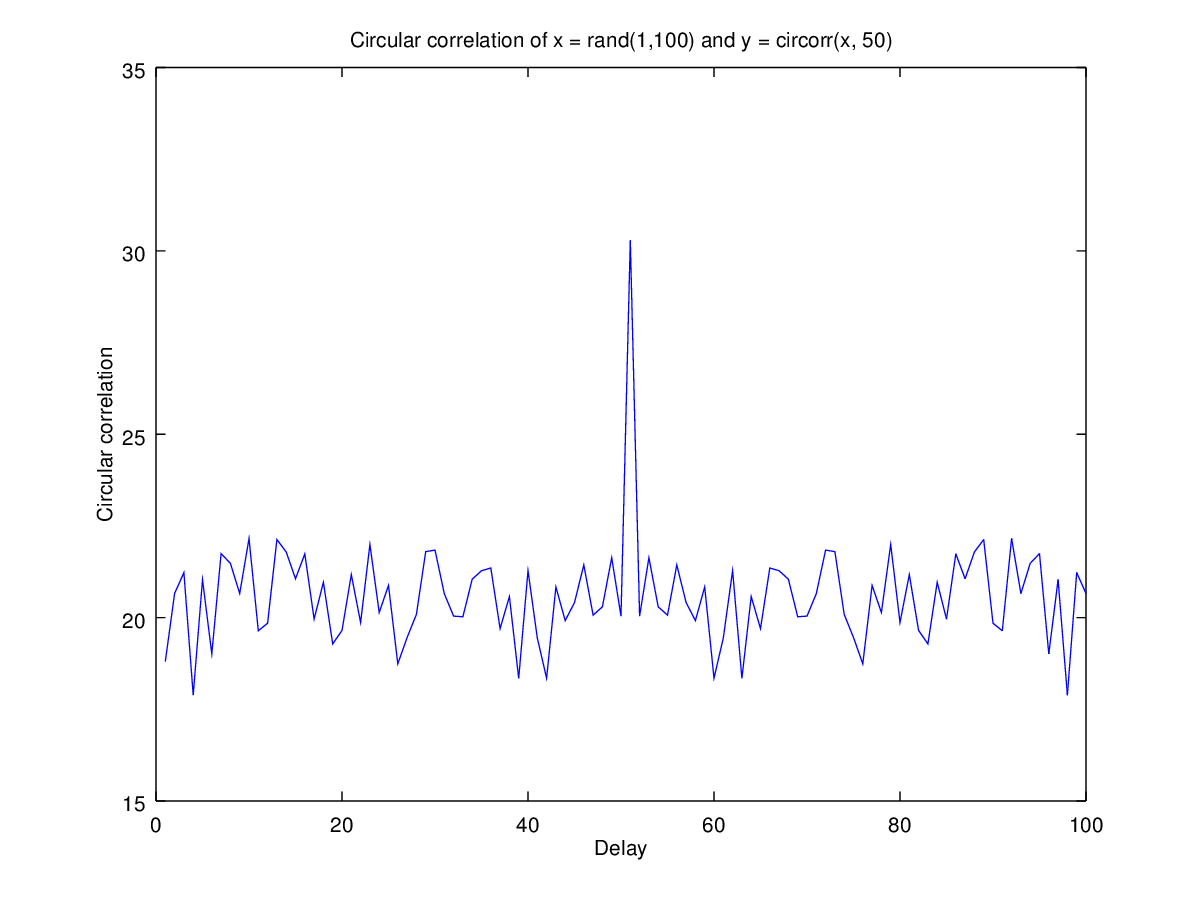
\includegraphics[width=.7\textwidth]{plot1c.png}
	\caption{The circular correlation between $x$ and itself.}
	\label{fig:1c}
\end{figure}

\subsection{}
See section \ref{code:1d} in the appendix for our implementation of the function $circpearson$. The following listing shows the results for two random 6-valued arrays $x$ and $y$. We can observe that the first values are the same (for a shift of 0). The subsequent values are reversed, because the functions `` shift'' in opposite directions.
\begin{lstlisting}[title=Results]
>>   pearson(x,y)
ans =

-0.59603   0.71090  -0.33988  -0.23198   0.90444  -0.44745

>>   circpearson(x,y)
ans =

-0.59603  -0.44745   0.90444  -0.23198  -0.33988   0.71090
\end{lstlisting}
The following listing shows the execution times for 10 runs of the functions. The table shows a great difference in execution times between the $pearson$ (total time of 0.005s) and $cirpearson$ (total time of 43.409s) functions.
\begin{lstlisting}[title=Speed]
#    Function Attr     Time (s)   Time (%)        Calls
----------------------------------------------------------
3 circpearson            39.377      90.70           10
41    binary +             1.714       3.95      5027000
43         mod             1.025       2.36      1250000
40    binary -             0.962       2.21      2526540
33    binary *             0.248       0.57      1275050
44        sqrt             0.048       0.11        50000
15   binary ==             0.019       0.04        50100
21      repmat             0.006       0.01           20
20    binary /             0.004       0.01        25070
34        mean             0.003       0.01           20
49         fft             0.002       0.00           20
45     pearson             0.002       0.00           10
5         lcm              0.002       0.00           10
51        ifft             0.001       0.00           10
13         all             0.001       0.00           70
31     reshape             0.001       0.00           40
39         sum             0.001       0.00           40
1        disp              0.000       0.00           10
2        rand              0.000       0.00           20
4      length              0.000       0.00          100

Top
1) circpearson: 10 calls, 43.409 total, 39.377 self
2) pearson: 10 calls, 0.005 total, 0.002 self
3) disp: 10 calls, 0.000 total, 0.000 self
4) rand: 20 calls, 0.000 total, 0.000 self
5) profile: 1 calls, 0.000 total, 0.000 self
\end{lstlisting}
In conclusion both functions yield the same results, but $pearson$ executes much faster, making it the preferable choice.

\subsection{}
A Pearson correlator is more useful in most applications because it returns an easily interpretable value that is normalized between -1 and 1, in contrast to the less intuitive values that a standard correlator returns.

\subsection{}
Figure \ref{fig:1f} gives the pearson correlation between sin(x) and cos(x) (plot1) and between 2sin(x) and cos(x). As we can see, the result is sin(x). This is the case, because at a delay of $0.5\pi$ the $cos(x)$ function is the same as the $sin(x)$ function, because $sin(x) = cos(x-.5\pi)$. As we can also observe, an amplitude difference does not yield different Pearson correlation coefficients. This is because the Pearson correlator normalizes the correlation coefficients between the range $[-1,1]$
\begin{figure}[H]
	\centering
	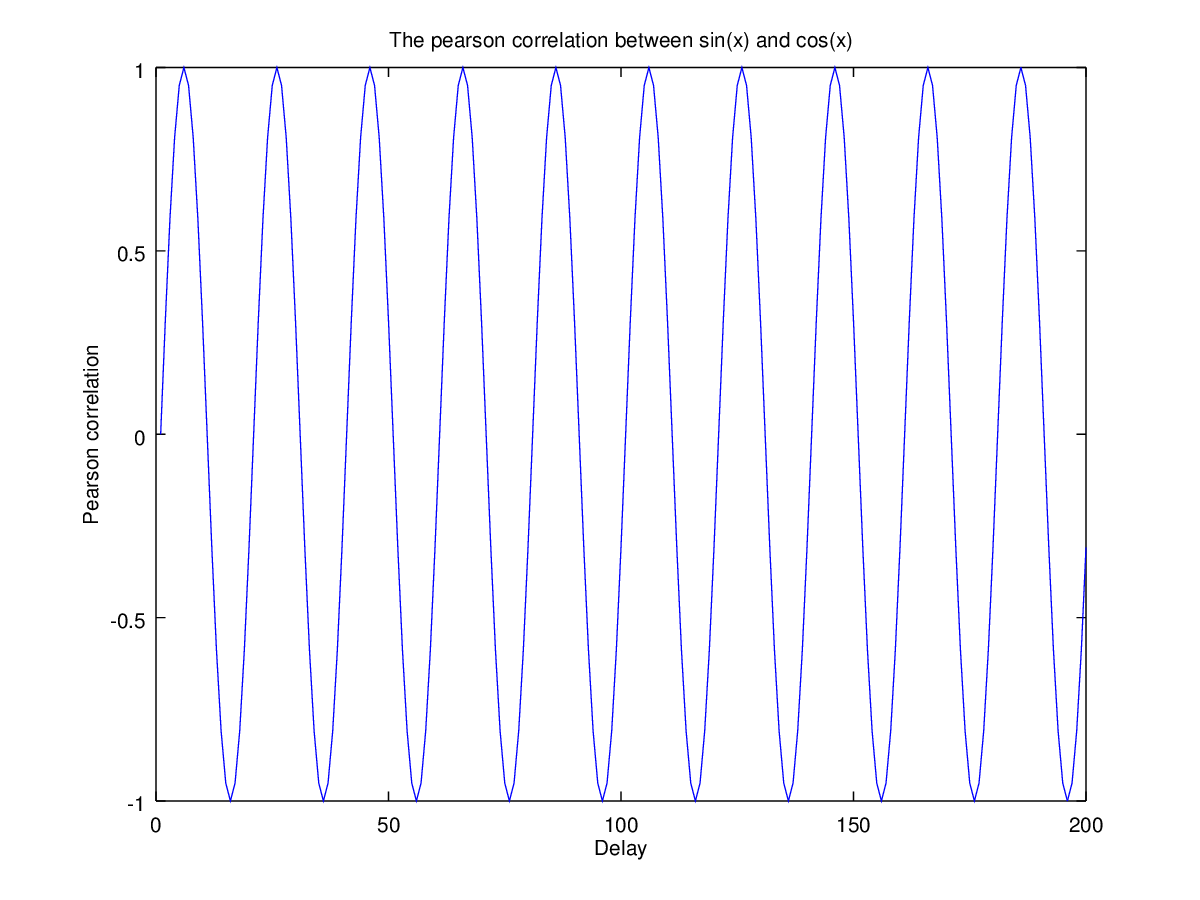
\includegraphics[width=.49\textwidth]{plot1f1.png}
	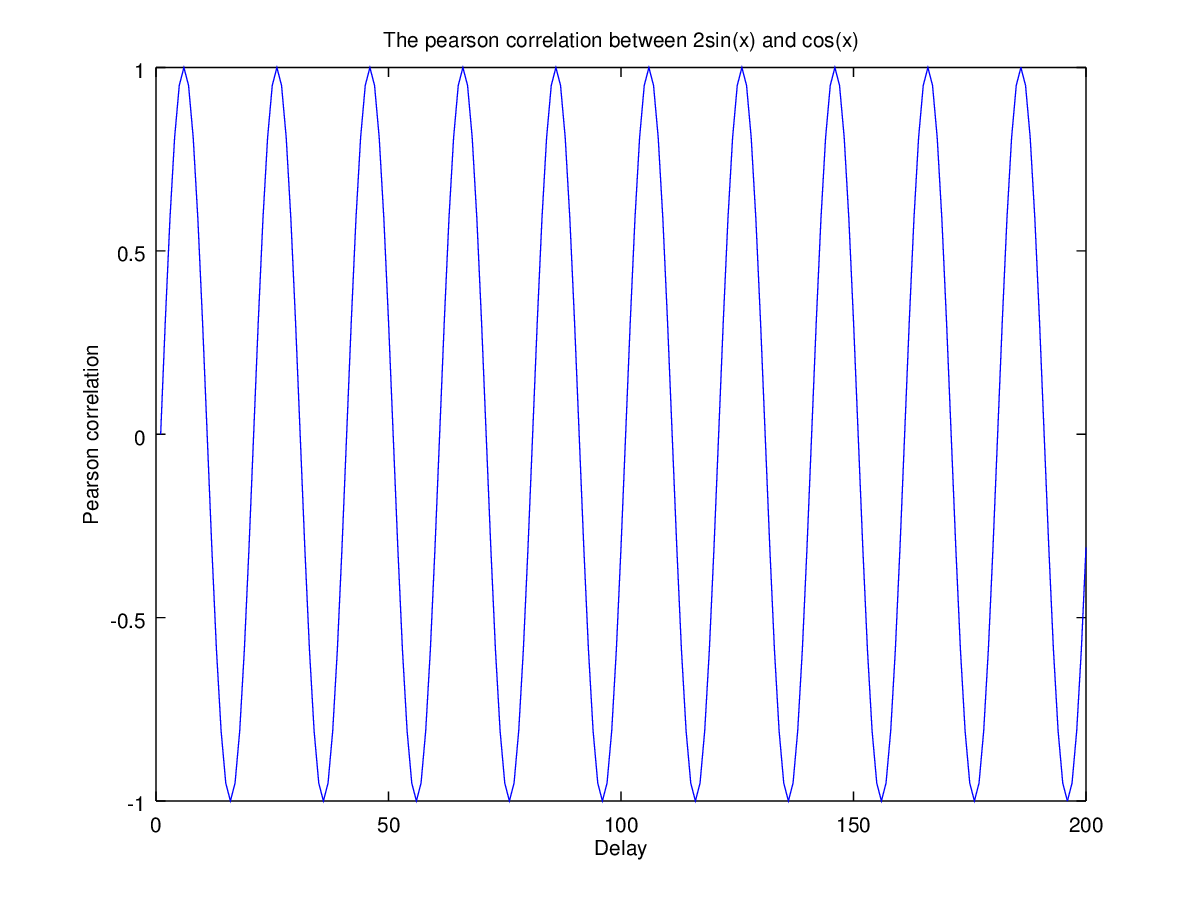
\includegraphics[width=.49\textwidth]{plot1f2.png}
	\caption{The pearson correlation between (1) sin(x) and cos(x), and (2) 2sin(x) and cos(x).}
	\label{fig:1f}
\end{figure}
\subsection{}
Figure \ref{fig:1g1} gives the plots of $x$, the Pearson correlation between $x$ and itself, and the Pearson correlation between $x$ and $y$. Furthermore plot \ref{fig:1g2} gives the Pearson correlation between $x$ and $y$ for six different noise levels. The noise was added using the function $x+i*(rand(1,100)*2-1)$, in which $x$ is the standard function $x$ and $i$ is the noise factor. The figure shows that up to a noise factor of around 1.2 you can still discriminate the peak at a delay of 50. A noise factor of 2 completely erases any observable trace of the old functions.
\begin{figure}[H]
	\centering
	\begin{subfigure}{0.49\textwidth}
		\centering
		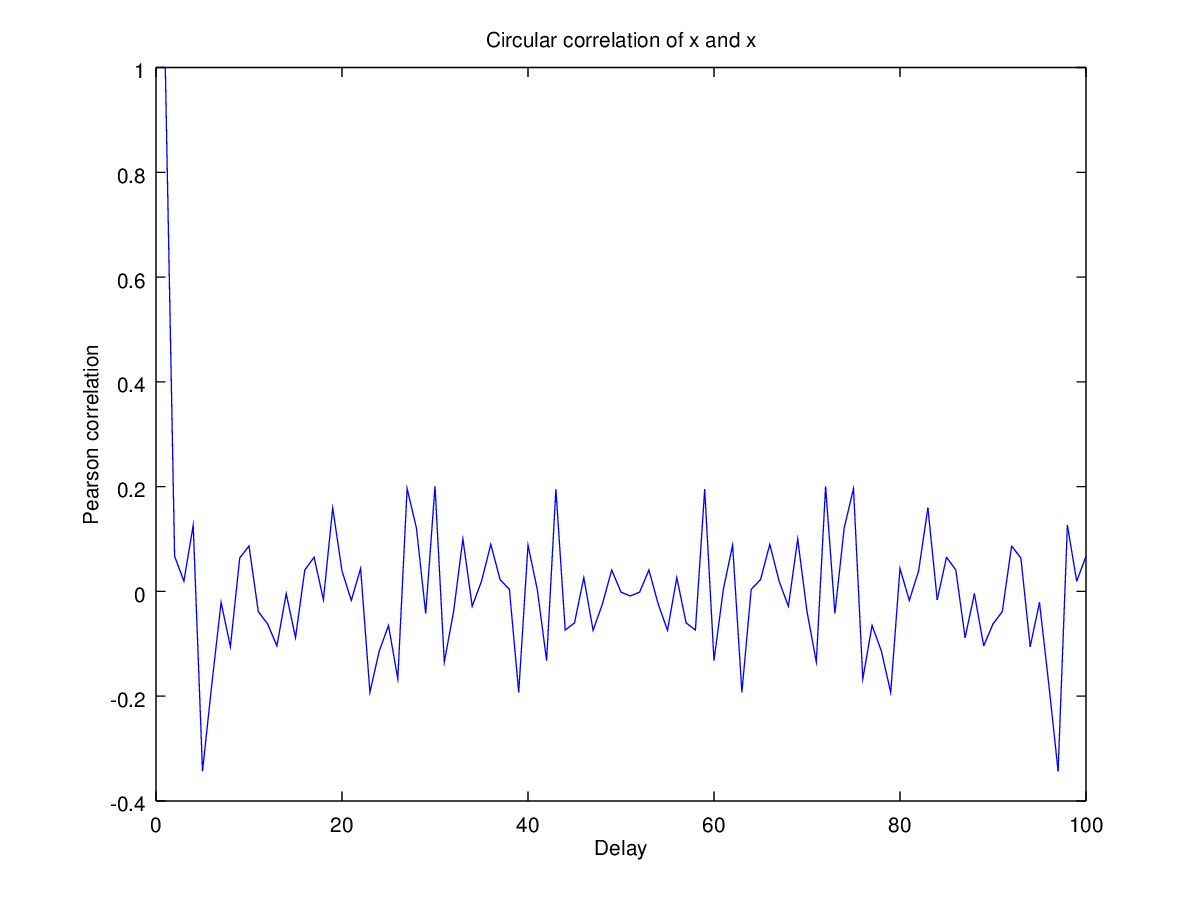
\includegraphics[width=\textwidth]{plot1ga.png}
		\caption{Function $x$.}
	\end{subfigure}
	\begin{subfigure}{0.49\textwidth}
		\centering
		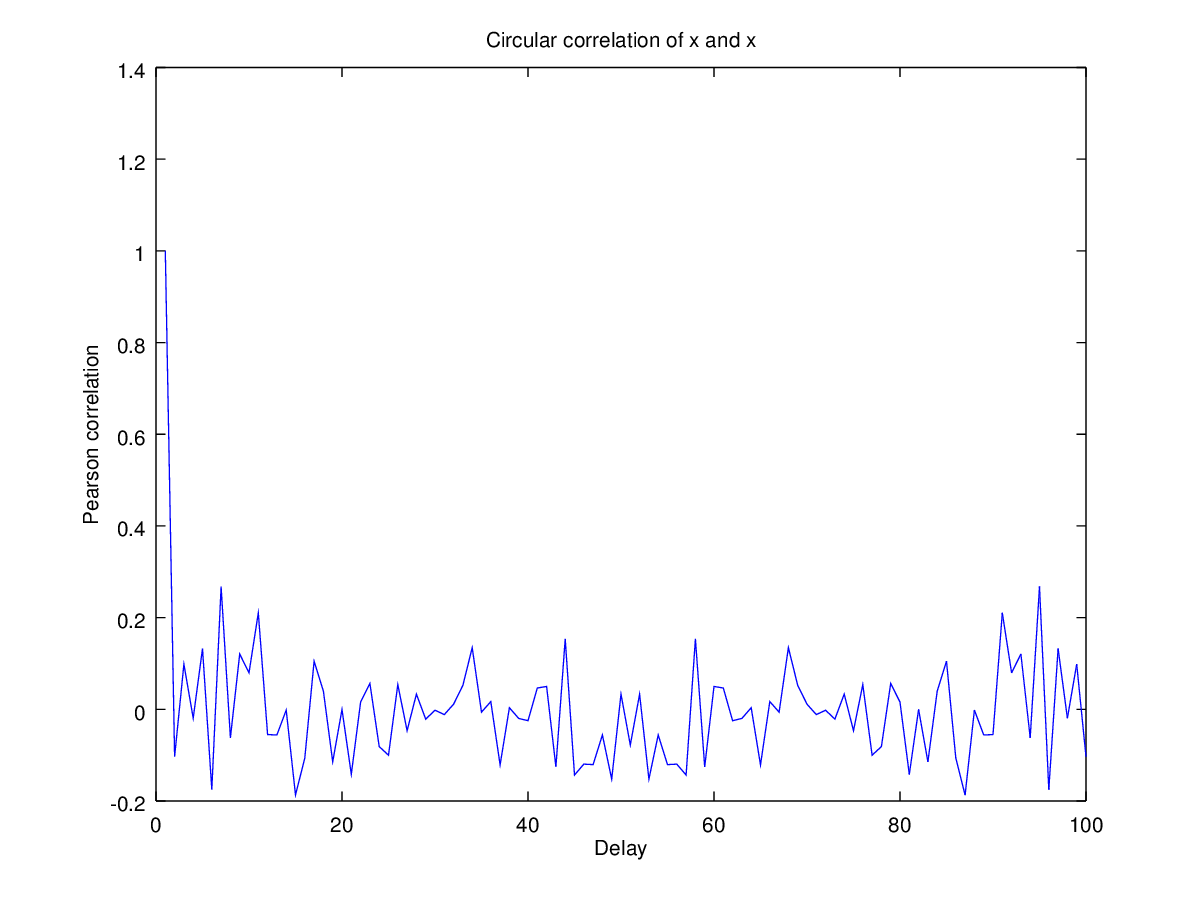
\includegraphics[width=\textwidth]{plot1gb.png}
		\caption{Pearson correlation between $x$ and $x$.}
	\end{subfigure}
	\begin{subfigure}{0.49\textwidth}
		\centering
		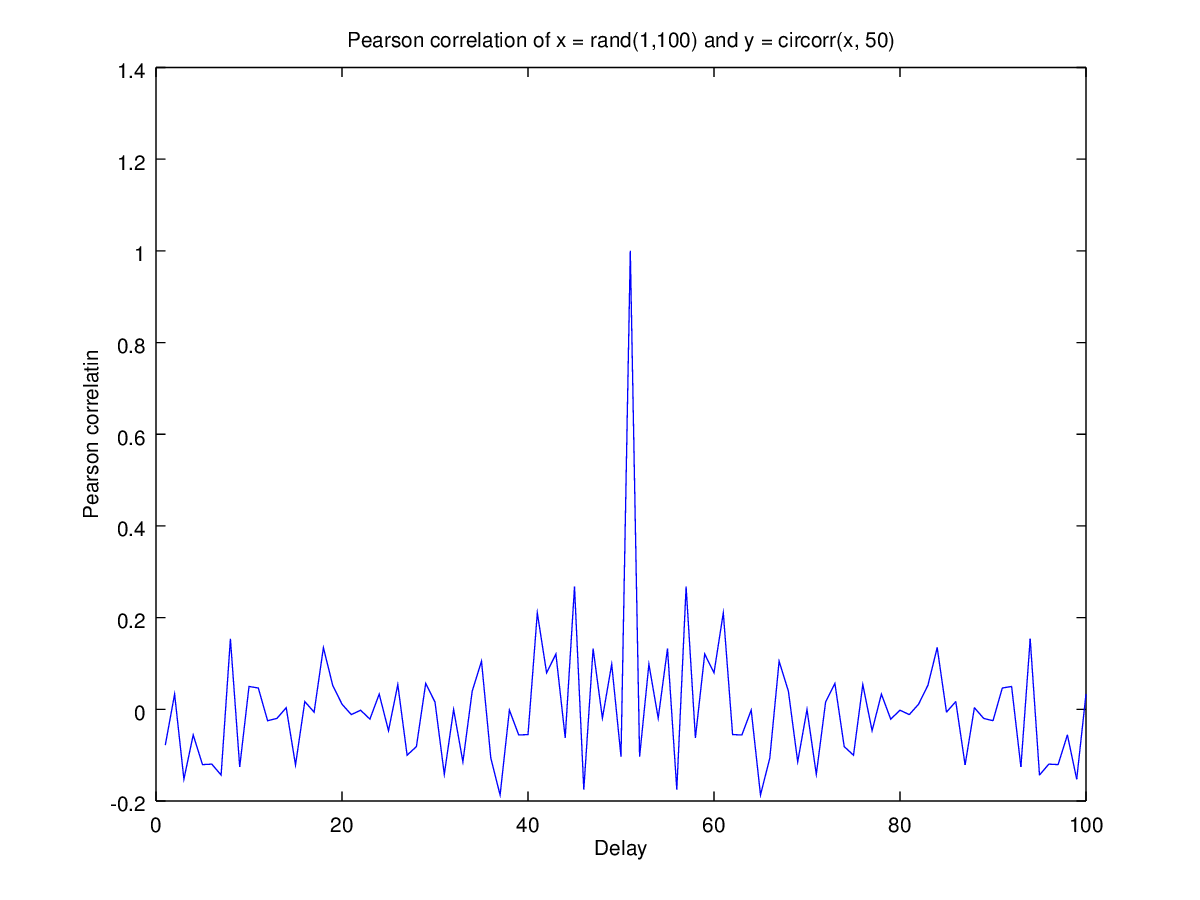
\includegraphics[width=\textwidth]{plot1gc.png}
		\caption{Pearson correlation between $x$ and $y$.}
	\end{subfigure}
	\caption{}
	\label{fig:1g1}
\end{figure}
\begin{figure}[H]
	\centering
	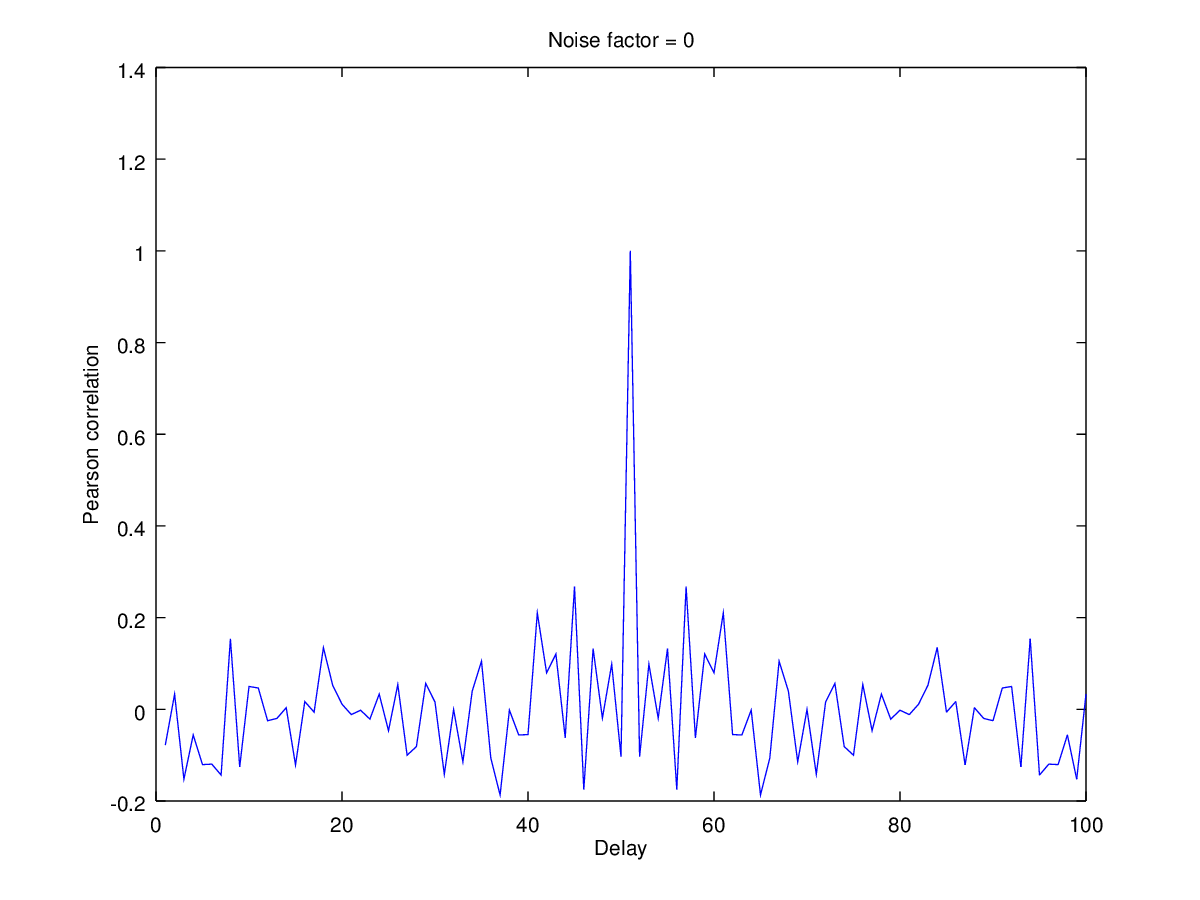
\includegraphics[width=.49\textwidth]{plot0noise.png}
	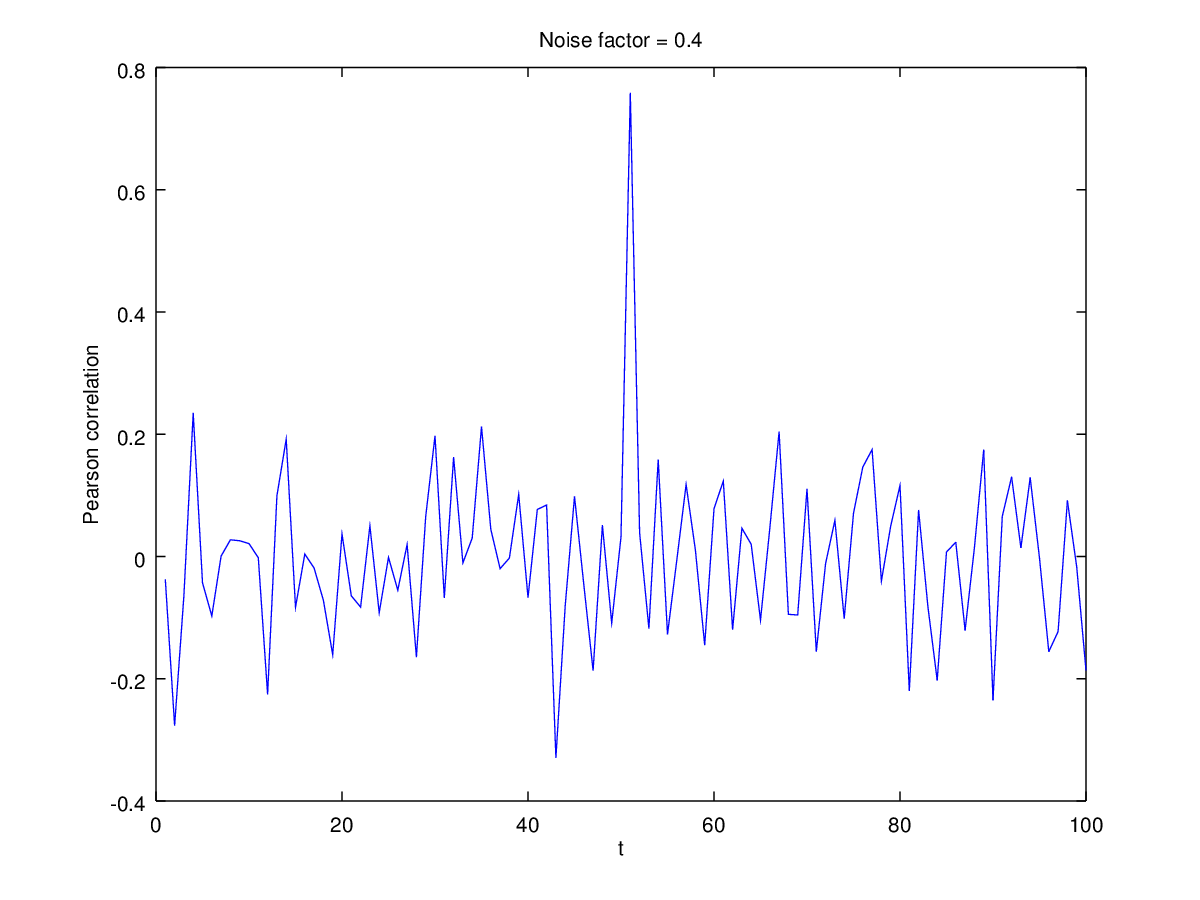
\includegraphics[width=.49\textwidth]{plot0_4noise}
	\\
	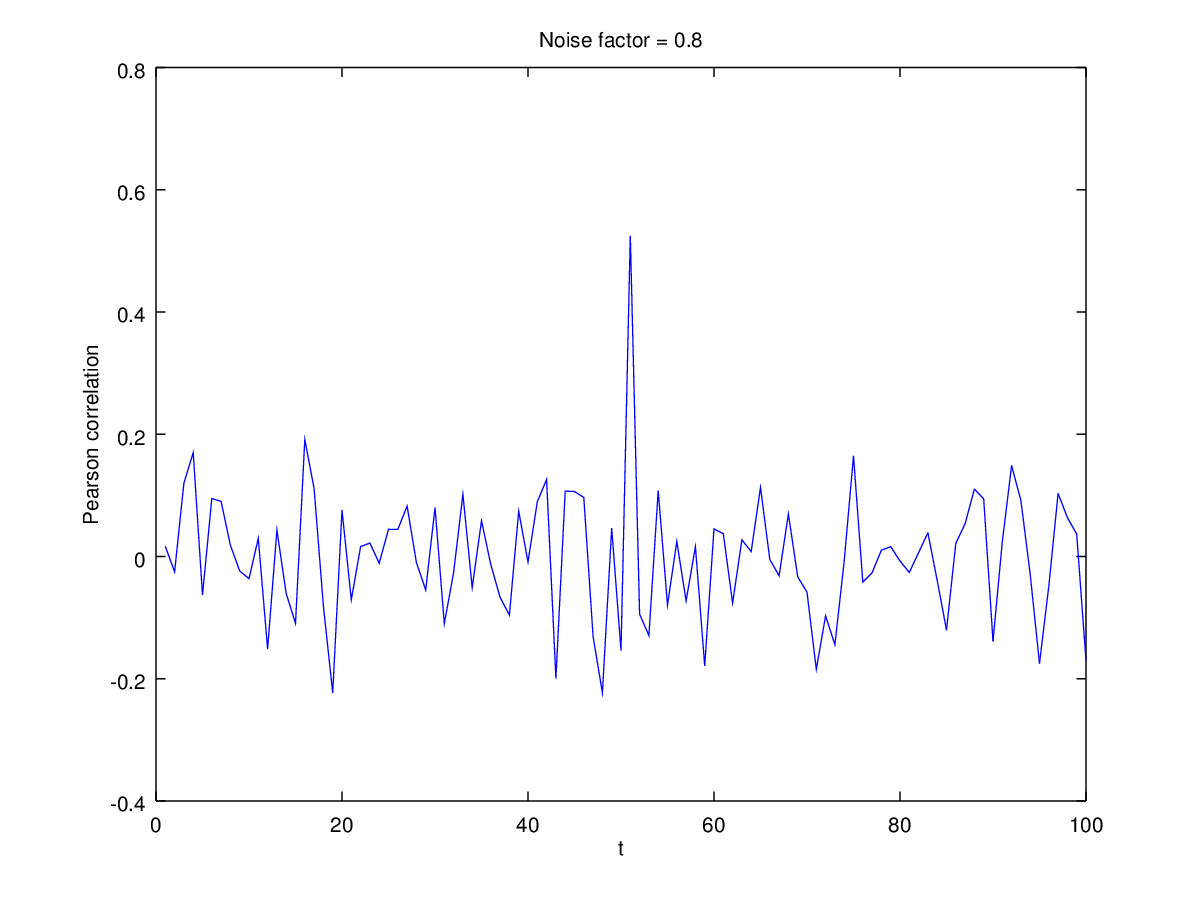
\includegraphics[width=.49\textwidth]{plot0_8noise}
	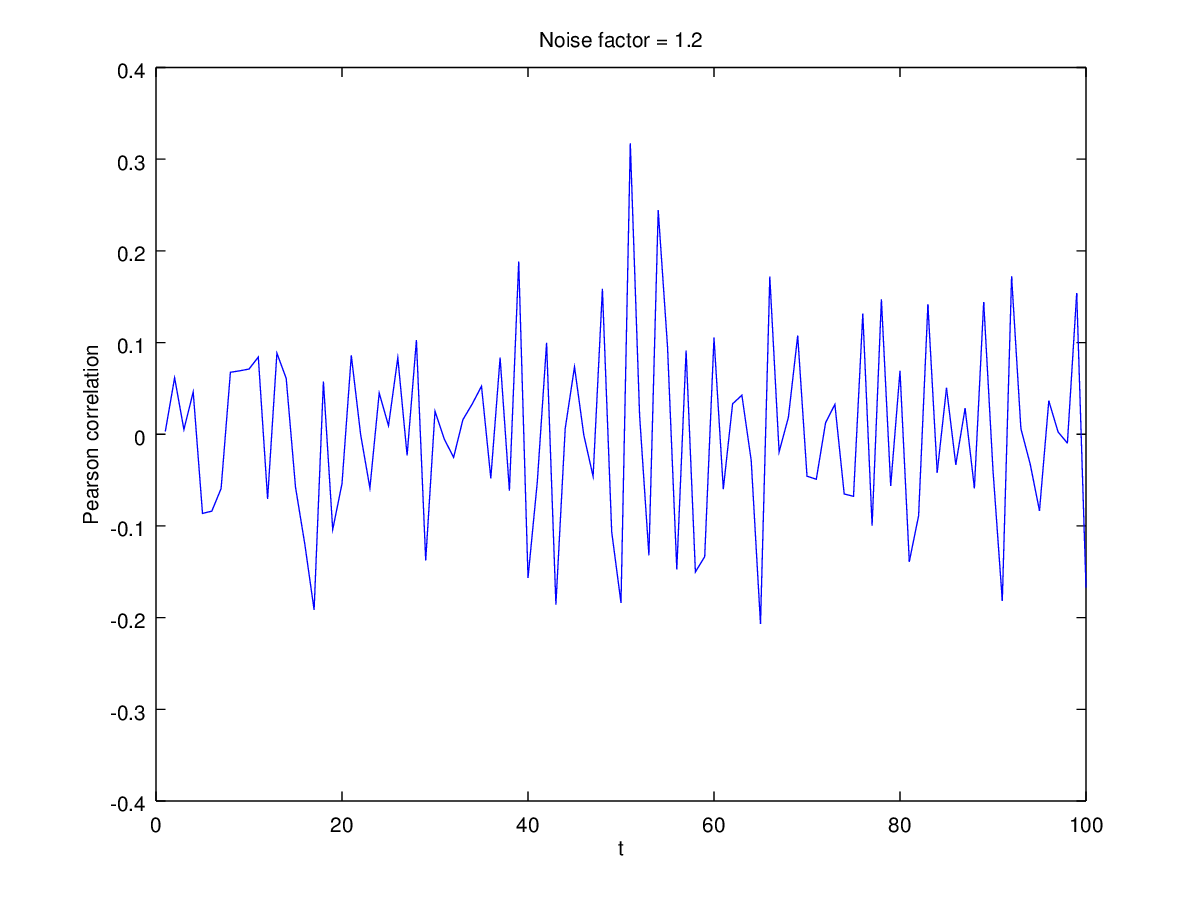
\includegraphics[width=.49\textwidth]{plot1_2noise}
	\\
	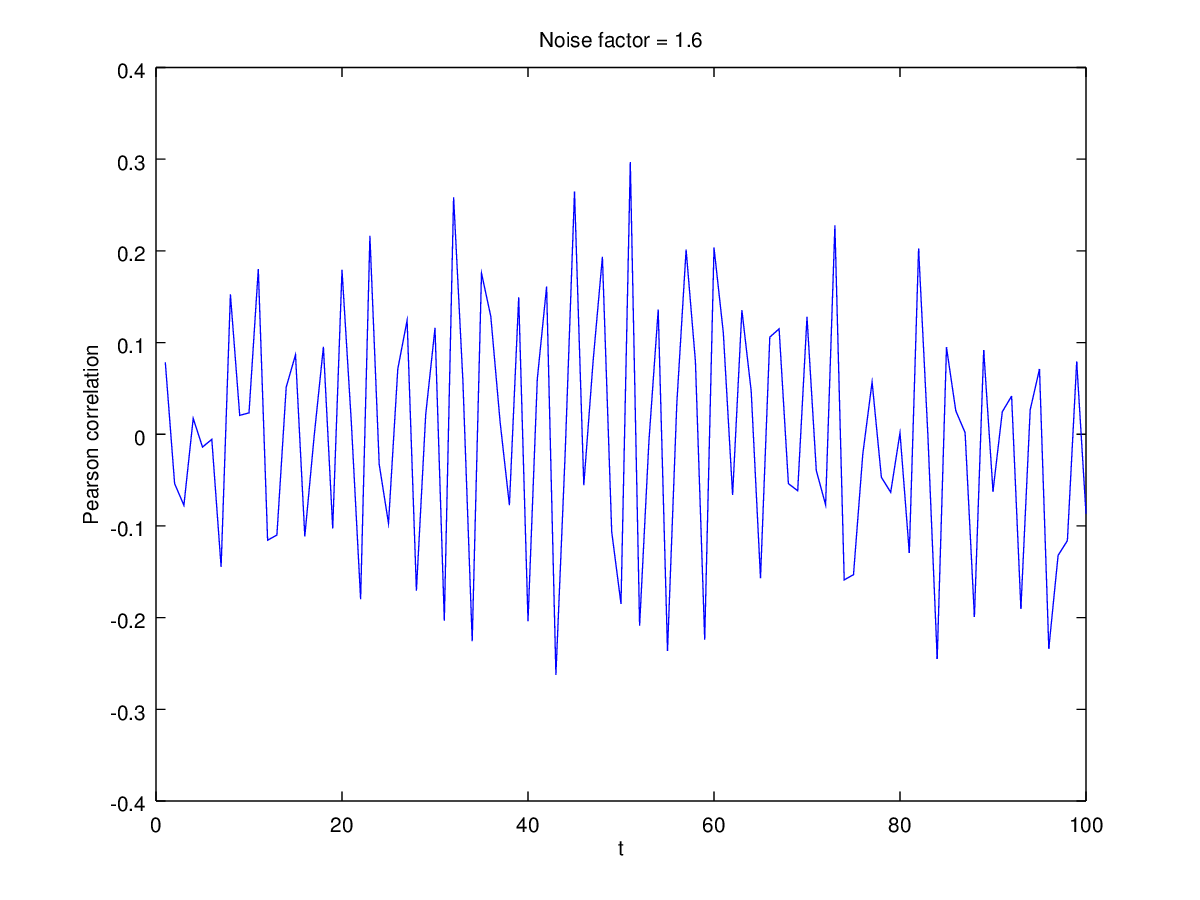
\includegraphics[width=.49\textwidth]{plot1_6noise}
	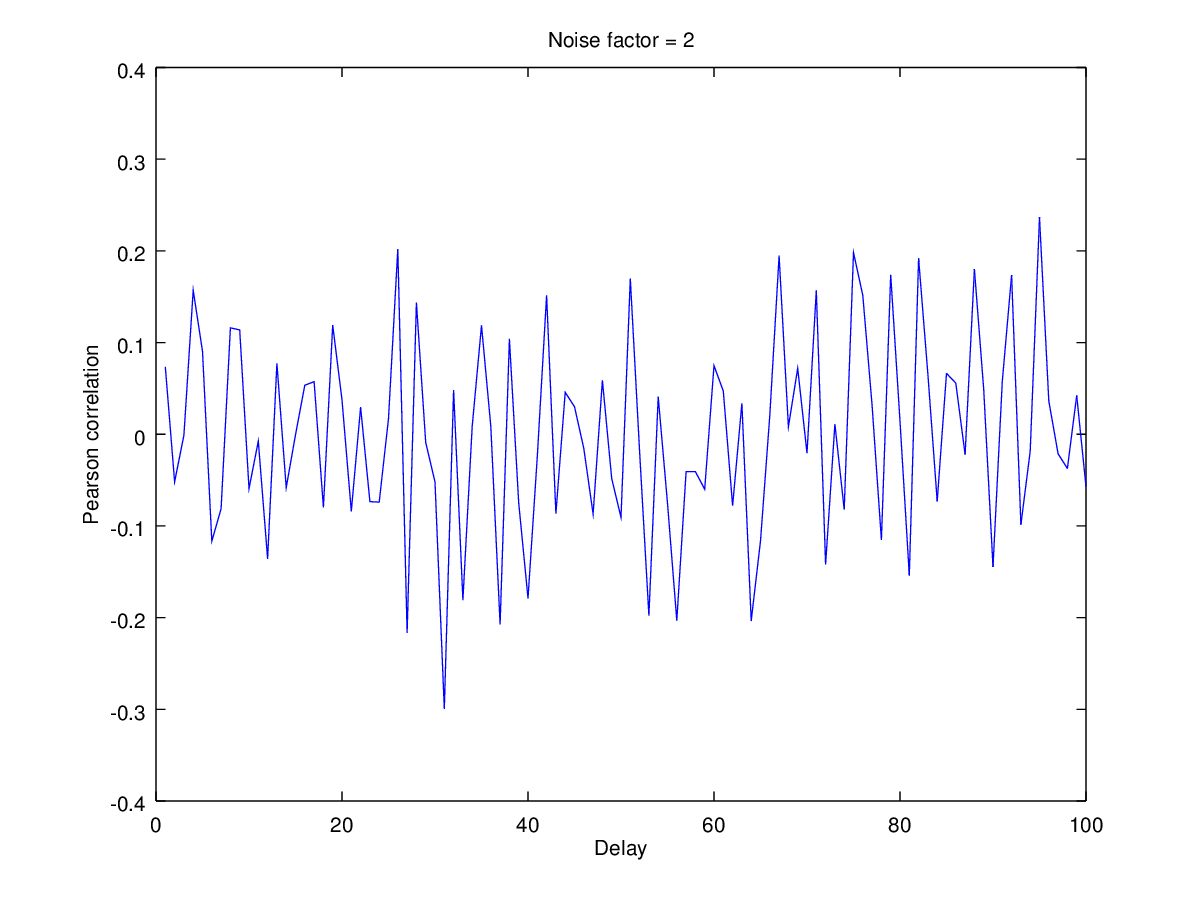
\includegraphics[width=.49\textwidth]{plot2noise.png}
	\caption{Pearson correlation between x and y, for different factors of noise added to x.}
	\label{fig:1g2}
\end{figure}

\section{A more general Pearson correlator}
\subsection{}
See Appendix~\ref{code:pearson2} for our implementation of the required function.

\subsection{}
Figure \ref{fig:2b} gives the function $x[n]$, the masks $h1[n]$ and $h2[n]$ and their
Pearson correlation with $x[n]$. We can conclude that the mask $h1$ is found exactly
in the signal $x[n]$, as there is a slice of $x[n]$ that has a Pearson correlation
of 1 with $h1$, whereas $h2$ is almost matched with a slice of $x[n]$, but not exactly
(a Pearson correlation of almost 1). So we conclude that $h1$ exists in $x[n]$, but
$h2$ does not.

\begin{figure}[H]
  \centering
  \begin{subfigure}{.52\textwidth}
    \centering
    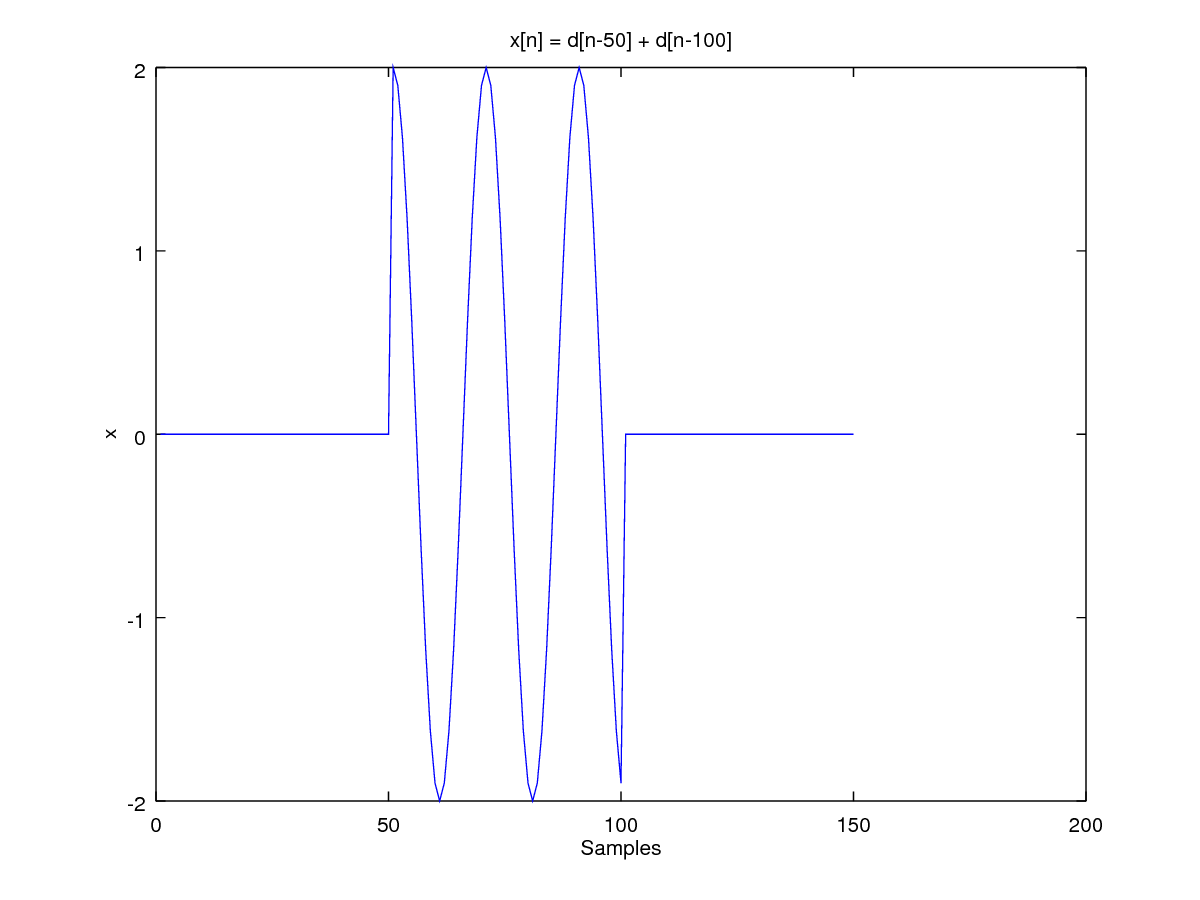
\includegraphics[width=\textwidth]{plot2b1.png}
    \caption{x[n]}
    \label{fig:2b1}
  \end{subfigure}
  \begin{subfigure}{.49\textwidth}
    \centering
    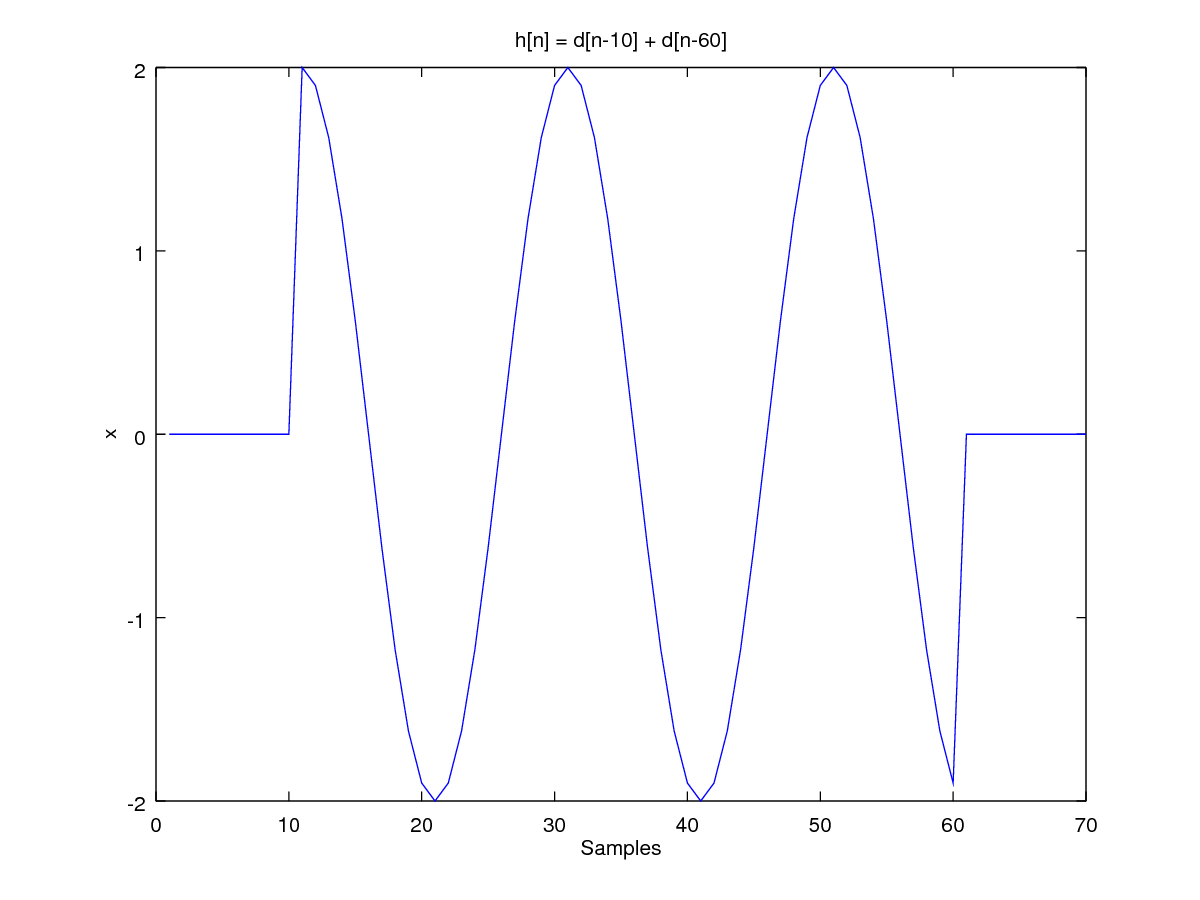
\includegraphics[width=\textwidth]{plot2b2.png}
    \caption{h1[n]}
    \label{fig:2b2}
  \end{subfigure}
  \begin{subfigure}{.49\textwidth}
    \centering
    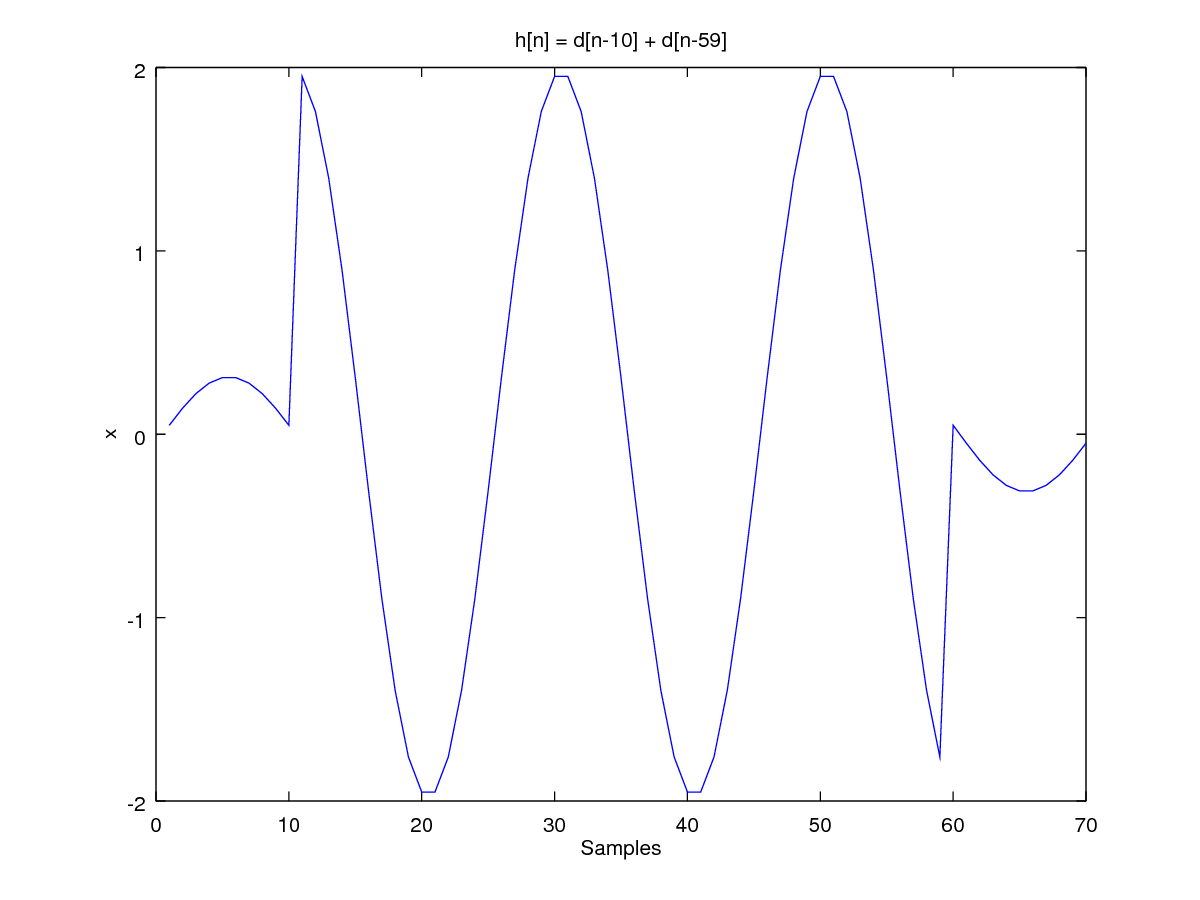
\includegraphics[width=\textwidth]{plot2b3.png}
    \caption{h2[n]}
    \label{fig:2b3}
  \end{subfigure}
  \begin{subfigure}{.49\textwidth}
    \centering
    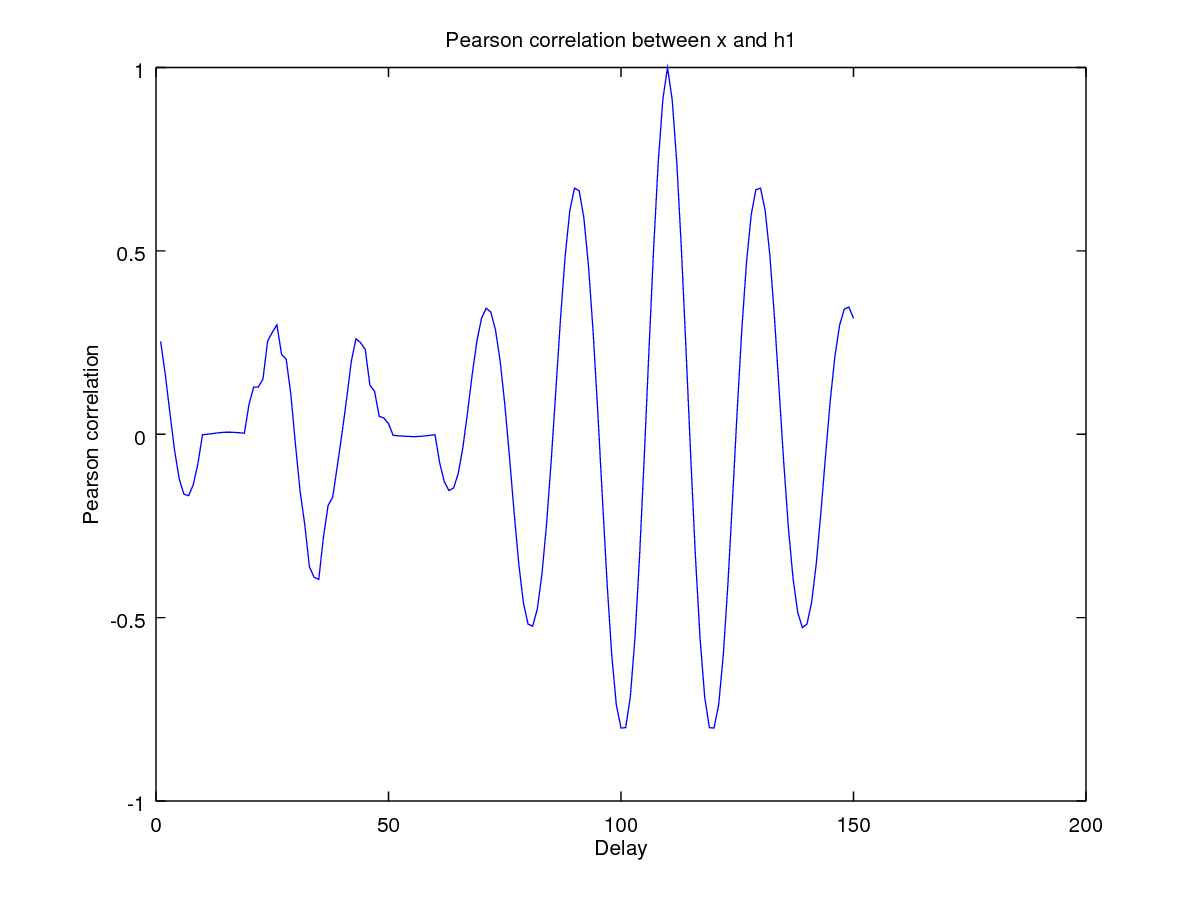
\includegraphics[width=\textwidth]{plot2b4.png}
    \caption{Pearson correlation between x[n] and h1[n].}
    \label{fig:2b4}
  \end{subfigure}
  \begin{subfigure}{.49\textwidth}
    \centering
    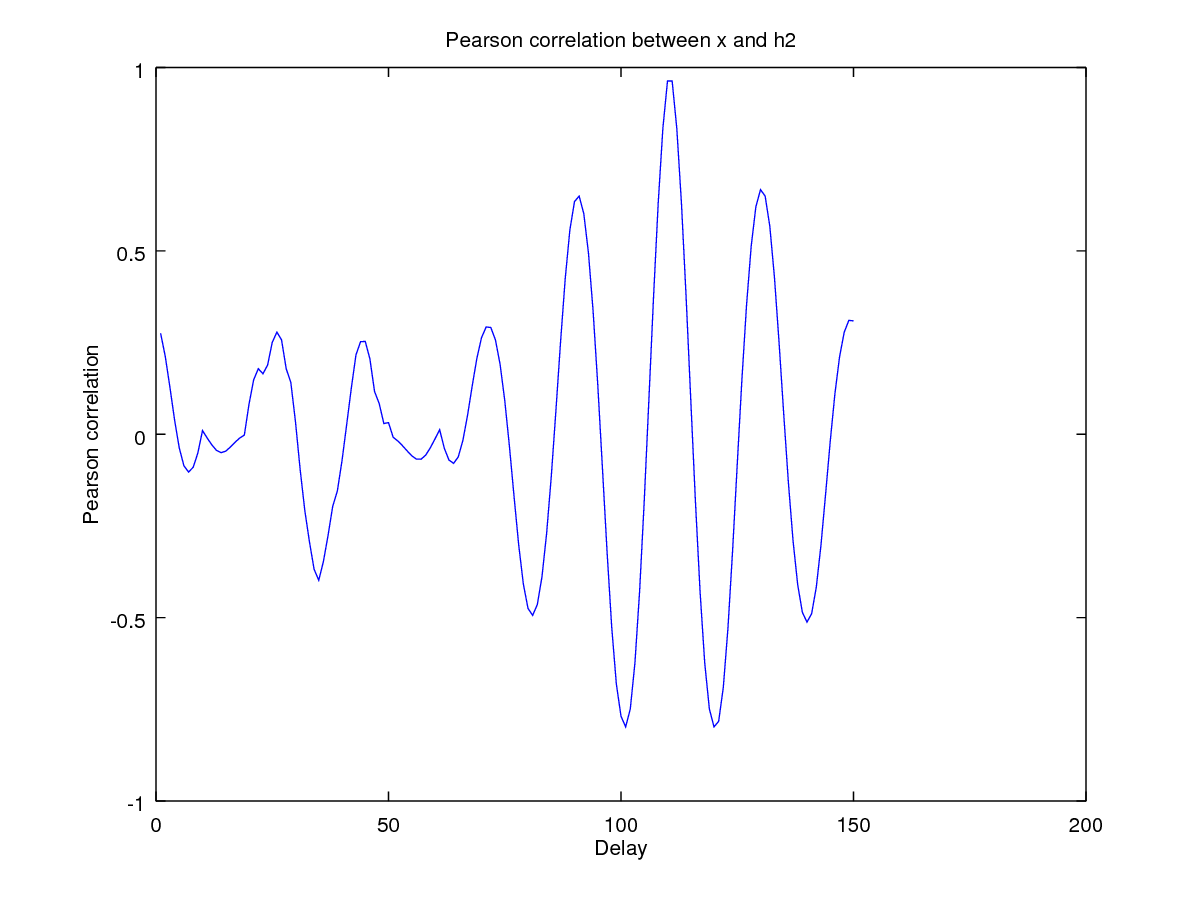
\includegraphics[width=\textwidth]{plot2b5.png}
    \caption{Pearson correlation between x[n] and h2[n].}
    \label{fig:2b5}
  \end{subfigure}
  \caption{}
  \label{fig:2b}
\end{figure}

\subsection{}
See Appendix~\ref{code:patternMatch} for our implementation of the function patternMatch.
Applying this function on x and h2 from the previous section, we acquire the plot
given in figure \ref{fig:2c}. From the figure we can observe the highest correlation value
in the given signal and check whether the mask can be foun in the actual given slice of signal,
not in the theoretical circular signal. In this specific case we can observe the highest
correlation at what seems to be sample 42. The correlation is not 1 though, which means
that the exact mask is not in the signal.
\begin{figure}[H]
  \centering
  \includegraphics[width=0.7\textwidth]{plot2c.pdf}
  \caption{The Pearson correlation for every subsequent slice of $x[n]$ and $h2$.}
  \label{fig:2c}
\end{figure}

\subsection{}
Figure \ref{fig:2d} gives the Pearson correlation between the mask hallelujah and
the signal handel. The figures shows that there is one exact match of the mask 'hallelujah'.
On the one han we can therefore conclude that this way of finding the mask works,
since it finds the exactly matching mask in the signal. On the other hand, this way
we do not find other occurences of the word 'hallelujah' that just are not completely
similar. If the word is only slightly pronounce differently or at another speed or
intensity, the correlation coefficient might be that much significantly lower, that
the occurence is not distinguishable from the other sound.
\begin{figure}[H]
  \centering
  \includegraphics[width=0.7\textwidth]{plot2d.pdf}
  \caption{The Pearson correlation for every slice of handel.wav and hallelujah.wav.}
  \label{fig:2d}
\end{figure}

\subsection{}
Figure \ref{fig:2e} gives the Pearson correlation between every subsequent slice of
the signal furelise and the mask cropelise. The figure shows multiple peaks, of which
one peak reaches the value 1, which signifies one slice being the exact same as the mask.
Furthermore we see more peaks reaching a correlation coefficient of approximately 0.5.
This indicates that there are multiple fragments in the signal which resemble the mask,
but are slightly different in some aspect(s). Therefore to detect the note pattern
of the musical interval, you could for example use an emperically determined threshold.
When a correlation coefficient is higher than the threshold, it is recognized as
the same musical pattern.
\begin{figure}[H]
  \centering
  \includegraphics[width=0.7\textwidth]{plot2e.pdf}
  \caption{The Pearson correlation for every slice of furelise8kHZ.wav and cropelise8kHZ.wav.}
  \label{fig:2e}
\end{figure}

\section{}

\begin{appendices}
\section{Code}
 \lstinputlisting[caption={circorr},label={code:1a}]{../code/circorr.m}
 \lstinputlisting[caption={1bc},label={code:1bc}]{../code/1bc.m}
 \lstinputlisting[caption={rotate},label={code:1c}]{../code/rotate.m}
 \lstinputlisting[caption={circpearson},label={code:1d}]{../code/circpearson.m}
 \lstinputlisting[caption={gensinusoid},label={code:gensinusoid}]{../code/gensinusoid.m}
 \lstinputlisting[caption={pearson2},label={code:pearson2}]{../code/pearson2.m}
 \lstinputlisting[caption={patternMatch},label={code:patternMatch}]{../code/patternMatch.m}
\end{appendices}
\end{document}
